\section{Introduction}
Lab 2 requires us to design and simulate an automatic windshield wiper with Ptolemy II, an open-source software developed by Berkeley for heterogeneous system design, modeling, and simulation.
\begin{center}
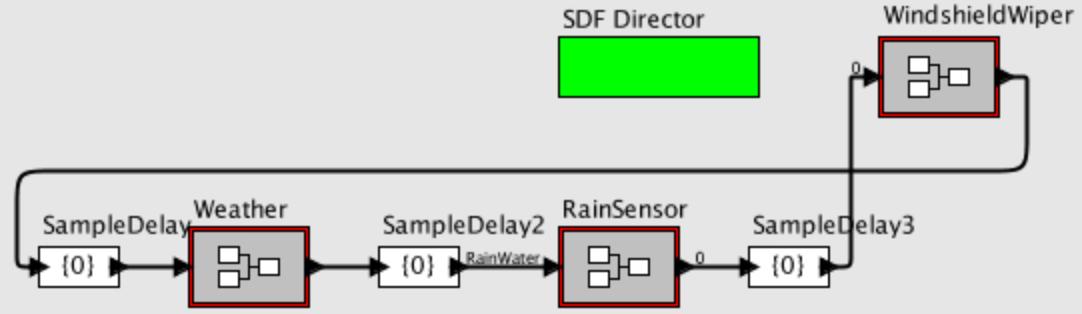
\includegraphics[width=12.5cm]{fig1.png}
\end{center}

\begin{center}
\small{Figure 1. Layout of the Automatic Windshield Wiper Model}
\label{layout}
\end{center}
As shown in Fig.1, the automatic windshield wiper model is consisted of three parts, the weather model that simulates weather conditions, the rain sensor model that detects raindrops on the surface of the windshield, and the windshield wiper model that receives rain sensor signals and controls the windshield wiper. 
\begin{center}
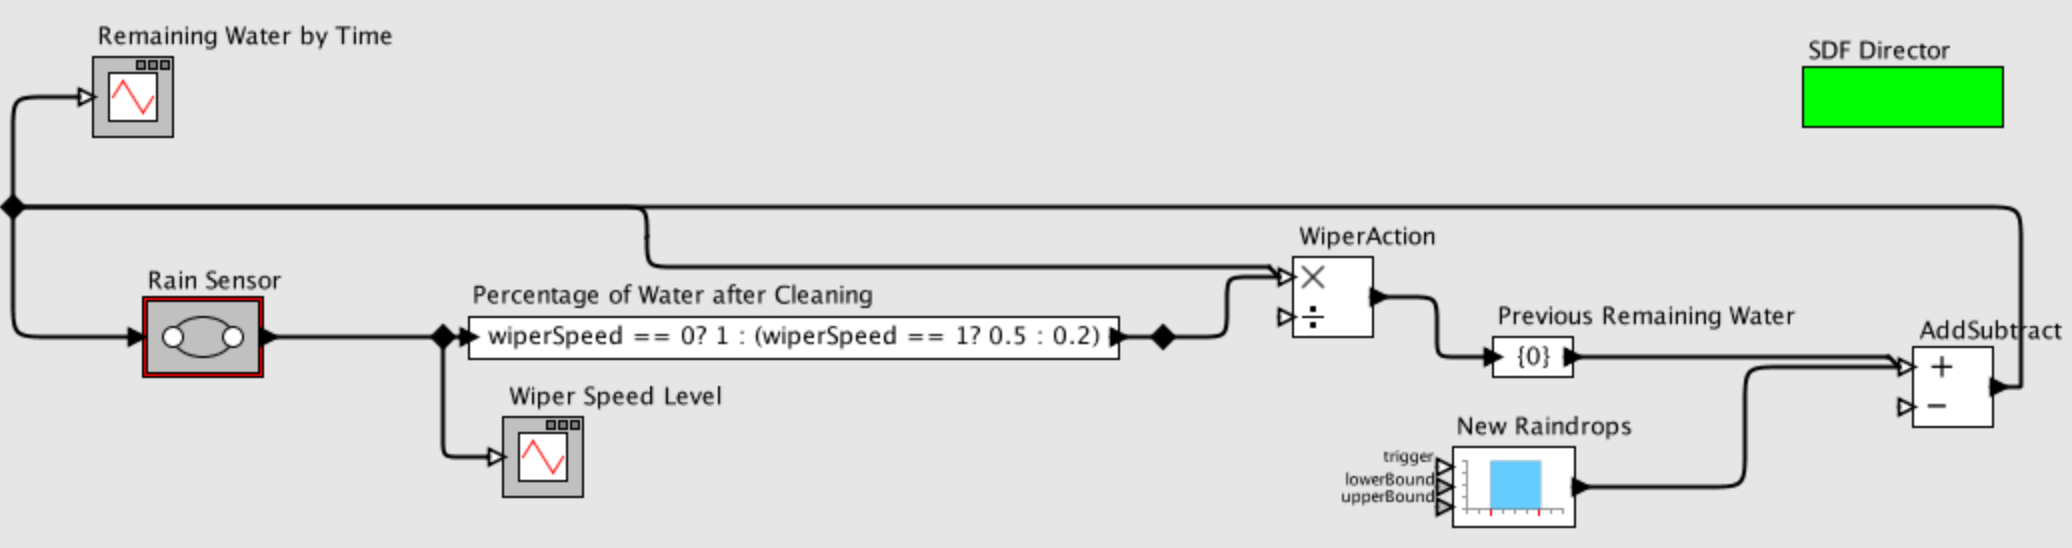
\includegraphics[width=13.5cm]{fig2.png}
\end{center}
\begin{center}
\small{Figure 2. Implementation of the Automatic Windshield Wiper Model}
\label{implementation}
\end{center}
A detailed implementation is shown in Fig.2, where the weather model is realized by a uniform random number generator, an adder, and a delay; the rain sensor model is realized by a finite state machine (FSM); the windshield wiper model is realized by an expression and a multiplier.